\documentclass[letterpaper]{article}
\usepackage[submission]{aaai2026}
\usepackage{times}
\usepackage{helvet}
\usepackage{courier}
\usepackage[hyphens]{url}
\usepackage{graphicx}
\urlstyle{rm}
\def\UrlFont{\rm}
\usepackage{natbib}
\usepackage{caption}
\frenchspacing
\setlength{\pdfpagewidth}{8.5in}
\setlength{\pdfpageheight}{11in}
\usepackage{amsmath}
\usepackage{amssymb}
\usepackage{booktabs}
\usepackage{algorithm}
\usepackage{algorithmic}

\pdfinfo{
/TemplateVersion (2026.1)
}

\title{Closed-form Second-order Data Shapley for Group Fairness:\\
Down-weighting Biased Training Examples Without Group Labels}
\author{Anonymous Submission}

\begin{document}
\maketitle

\begin{abstract}
A model trained by empirical risk minimization inherits the biases in its data:
when a majority group ties an attribute to the label, the model uses that
biased attribute and becomes \emph{unfair} to the minority group. We ask whether
\emph{closed-form data valuation} can prevent this during training, with no group
labels in the model update. We repurpose In-Run Data Shapley \citep{wang2024inrun}
as an in-training per-sample reweighter, and add an RMS-rescaled second-order
gradient--Hessian--gradient cross-term. The cross-term \emph{automatically
down-weights biased-majority examples} (on a controlled probe, majority Shapley
values are lower than minority, $p=1.89\times10^{-8}$), and a residual ablation
shows this comes from a real directional signal, not from smoothing. Across three
data-bias regimes --- color, texture, and natural images --- the method improves
worst-group accuracy and \textbf{shrinks the majority--minority accuracy gap by
$40$--$47\%$ over ERM}, and it beats a bi-level fairness reweighter
\citep{ren2018reweight}, among methods that use \emph{no group labels} at training
(stronger group-label / two-stage methods exist, which we report). On \textbf{CelebA}
--- a structured \emph{image} demographic bias (predict blond hair, sensitive
group gender) --- it lifts worst-group accuracy by $+51$~pp and cuts the
equalized-odds gap $0.38{\to}0.16$; on \emph{diffuse} tabular data (Adult, COMPAS)
the gain is small. The mechanism needs structured bias.
\end{abstract}

\section{Introduction}

Fairness problems in machine learning often start in the \emph{data}. If, in the
training set, a majority group links some attribute to the label --- background to
object, color to digit, a demographic feature to an outcome --- a model trained to
minimize average loss will happily use that attribute. Average accuracy looks
good, but the model has \emph{learned the bias}, and it fails on the group where
the attribute does not hold. This is exactly an unfair model: it works well for
the well-represented group and poorly for the under-represented one. In high-stakes uses --- lending,
hiring, medical triage --- this becomes discrimination: the model is least
reliable for the group that is already least represented. Resisting data bias
\emph{during} training, rather than patching the model afterward, is a core
fairness goal.

The strongest fairness fixes assume extra supervision: group labels at training
time (GroupDRO, \citealp{sagawa2020groupdro}), a second training stage
\citep{liu2021jtt}, or a bi-level meta-loop \citep{ren2018reweight}. We ask a
different question: \emph{can a closed-form, single-pass signal --- computed during
ordinary training, with no group labels in the update --- tell us which examples
are teaching the bias, so we can down-weight them?}

Our starting point is In-Run Data Shapley \citep{wang2024inrun}, which gives a
closed-form estimate of how much each training example helps a small, balanced
reference set, \emph{during} the run. We turn this valuation into a per-sample
weight, and study what its \emph{second-order} (curvature) term adds. We find the
curvature term is the part that targets the bias.

This connects two course themes --- data valuation and group fairness --- by
turning a \emph{valuation} estimator into a \emph{bias-mitigation} signal inside
the optimizer. Our contributions:
\begin{itemize}\setlength{\itemsep}{1pt}
\item A closed-form In-Run Data Shapley reweighter for \textbf{fair training}: it
down-weights examples that teach data bias, using no group labels in the update.
\item A second-order gradient--Hessian--gradient cross-term with \textbf{RMS
rescaling}, required for stability under strong bias.
\item A \textbf{residual ablation} proving the bias-correcting signal is a real,
sample-specific direction (the orthogonal residual), not smoothing.
\item Across \textbf{three data-bias regimes} the method raises worst-group
accuracy and shrinks the majority--minority gap by $40$--$47\%$ over ERM.
\item An \textbf{honest scope}: a controlled probe of the mechanism, a clean
boundary on diffuse tabular demographic bias, and plainly stronger baselines.
\end{itemize}

\section{Related Work}

\paragraph{Group fairness and worst-group accuracy.}
A common operational notion of group fairness is high \emph{worst-group} accuracy
and a small gap between groups \citep{sagawa2020groupdro}. GroupDRO uses group
labels; JTT \citep{liu2021jtt} and IRM \citep{arjovsky2019irm} relax that need.
These are strong but heavier; we offer a closed-form alternative and report the
gap honestly.

\paragraph{Fairness by reweighting.}
Learning to reweight \citep{ren2018reweight} and FORML \citep{yan2022forml} solve
a bi-level meta problem; ARL \citep{lahoti2020arl} reweights adversarially without
demographics. Our reweighter is closed-form and single-pass --- no inner loop.

\paragraph{Data valuation.}
Data Shapley \citep{ghorbani2019datashapley} values examples by marginal
contribution but needs many retrainings; In-Run Data Shapley \citep{wang2024inrun}
makes it closed-form in one run. FairShap \citep{arnaiz2023fairshap} uses Shapley
values for \emph{fair data valuation}; we instead inject a second-order Shapley
signal into the optimization trajectory to mitigate bias as it is being learned.

\section{Method: Fairds}
\label{sec:method}

\paragraph{Setup.}
At step $t$ with parameters $\theta_t$, a minibatch $\mathcal{B}=\{z_i\}_{i=1}^B$
and a small \emph{group-balanced anchor} $\mathcal{D}_{\mathrm{val}}$ (50:50;
group labels are used only to build the anchor once, never in the model update).
Let $g_i=\nabla_\theta L(z_i;\theta_t)$ and
$g_{\mathrm{val}}=\nabla_\theta L(\mathcal{D}_{\mathrm{val}};\theta_t)$.

\paragraph{First order.}
$\phi_i^{(1)}=\langle g_i,g_{\mathrm{val}}\rangle$ \citep{wang2024inrun} measures
how much $z_i$ reduces loss on the balanced anchor in one SGD step. Per-sample
gradients use \texttt{torch.func.vmap} in a single graph --- closed form, no
bi-level loop.

\paragraph{Second order with RMS rescaling.}
We add the gradient--Hessian--gradient cross-term
$c_i=\langle g_i, H_{\mathrm{val}}\,g_{\mathrm{val}}\rangle$, with
$H_{\mathrm{val}}\,g_{\mathrm{val}}$ from the Pearlmutter trick
\citep{pearlmutter1994hvp} (one extra backward pass, no explicit Hessian). Since
the spectrum of $H_{\mathrm{val}}$ varies by orders of magnitude, a fixed
$\alpha$ is unusable; we \textbf{rescale the cross-term to the same RMS magnitude
as the first-order term} each minibatch:
\begin{equation}
\widetilde\phi_i^{(2)} = \phi_i^{(1)} - \alpha\,
\frac{\mathrm{RMS}(\phi^{(1)})}{\mathrm{RMS}(c)}\; c_i .
\label{eq:phi2}
\end{equation}
Without this rescaling, the method collapses to chance under strong bias.
Examples with low $\widetilde\phi$ --- those that help the biased majority but not
the balanced anchor --- are down-weighted.

\begin{algorithm}[t]
\caption{Fairds reweighting step (second order)}
\label{alg:fairds}
\begin{algorithmic}[1]
\REQUIRE minibatch $\mathcal{B}$, balanced anchor $\mathcal{D}_{\mathrm{val}}$,
params $\theta_t$, EMA buffer $e$, scalars $\alpha,\tau$
\STATE $g_i \leftarrow \nabla_\theta L(z_i;\theta_t)$ for $z_i\in\mathcal{B}$
\hfill {\footnotesize\textit{// vmap, single graph}}
\STATE $g_{\mathrm{val}}\leftarrow\nabla_\theta L(\mathcal{D}_{\mathrm{val}};\theta_t)$;\;\;
$Hg\leftarrow$ Pearlmutter$(\theta_t,g_{\mathrm{val}})$
\STATE $\phi^{(1)}_i\leftarrow\langle g_i,g_{\mathrm{val}}\rangle$;\;\;
$c_i\leftarrow\langle g_i,Hg\rangle$
\STATE $\widetilde\phi_i\leftarrow\phi^{(1)}_i-\alpha\,
\frac{\mathrm{RMS}(\phi^{(1)})}{\mathrm{RMS}(c)}\,c_i$
\hfill {\footnotesize\textit{// RMS rescale}}
\STATE $e_i\leftarrow\mathrm{EMA}(e_i,\widetilde\phi_i)$;\;\;
$w\leftarrow B\cdot\mathrm{softmax}(e_{\mathcal{B}}/\tau)$, clipped
\STATE $\theta_{t+1}\leftarrow\theta_t-\eta\sum_{i}w_i\,\nabla_\theta L(z_i;\theta_t)$
\end{algorithmic}
\end{algorithm}

\paragraph{Stabilizers.}
Two choices make the reweighter robust. The EMA buffer averages each example's
score over the steps where it appears, so one noisy minibatch cannot dominate its
weight. The per-batch softmax weights are clipped at quantile bounds, so no
example collapses to zero or explodes --- important under strong bias, where a few
majority examples would otherwise be driven to negligible weight.

\paragraph{Why the cross-term targets bias.}
$g_{\mathrm{val}}$ is nearly the top eigenvector of $H_{\mathrm{val}}$ (alignment
$0.89$--$0.99$), so the normalized cross-term $c_n$ is almost parallel to
$\phi^{(1)}$. Decomposing $c_n=\beta\,\phi^{(1)}+r$ separates a \emph{parallel}
part (a global shrinkage, like smoothing) from an \emph{orthogonal residual} $r$.
Whether $r$ is a real bias signal is tested in Section~\ref{sec:residual}.

\section{Experiments}

We measure group fairness three ways: \textbf{worst-group accuracy} (higher is
fairer; the max--min notion), the \textbf{group accuracy gap} between the
biased-majority and the minority group (lower is fairer), and, for tabular data,
the \textbf{demographic-parity (DP)} and \textbf{equalized-odds (EO)} gaps. We
compare Vanilla SGD; our Fairds-1/2 and the residual variant; a corrected one-step
bi-level reweighter (\citealp{ren2018reweight}, a FORML proxy); JTT
\citep{liu2021jtt}; and GroupDRO \citep{sagawa2020groupdro}. Vanilla, Fairds,
Ren2018 and JTT use \emph{no group labels} in the update; GroupDRO uses them.

\begin{figure*}[t]
\centering
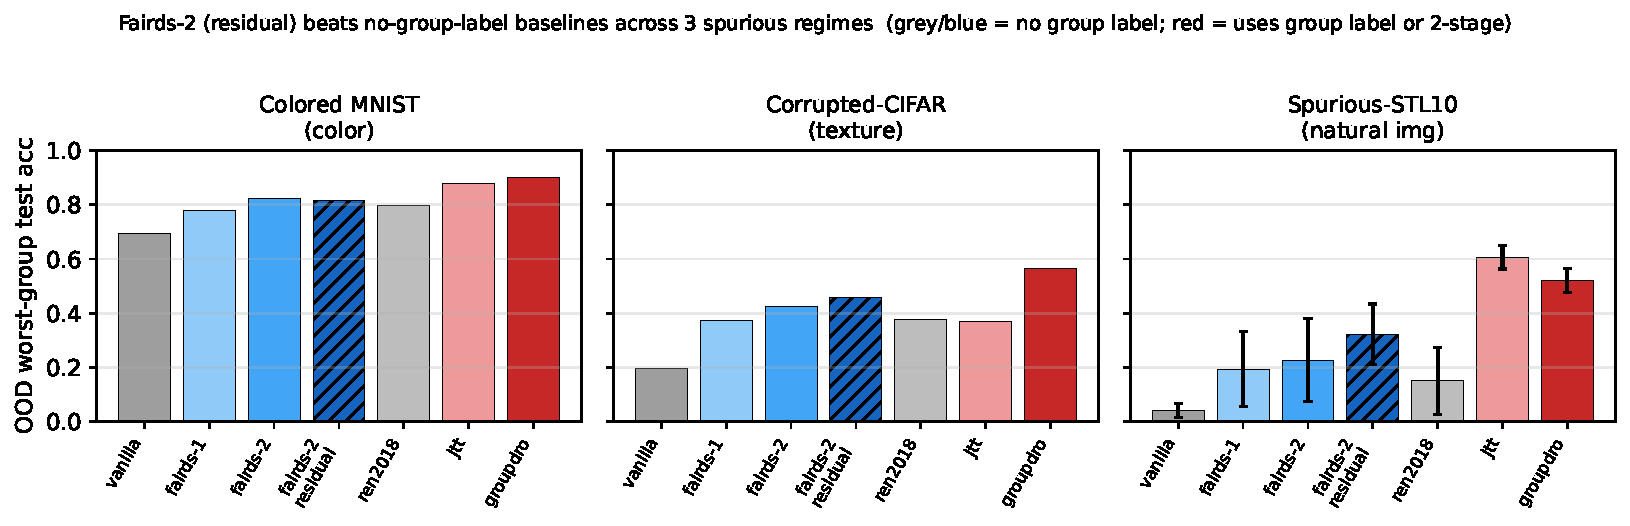
\includegraphics[width=0.97\textwidth]{figures/fig_three_regimes.pdf}
\caption{\textbf{Group fairness across three data-bias regimes.} Worst-group
accuracy (higher = fairer). Grey/blue bars use \emph{no} group label at training;
red bars use a group label or a two-stage procedure. The second-order residual
variant (hatched) protects the under-represented group better than every
no-group-label baseline, in all three regimes. STL10 error bars are $\pm1$ std
(10 seeds).}
\label{fig:three}
\end{figure*}

\subsection{Setup}
\label{sec:setup}
Three from-scratch image benchmarks share one bias structure and differ only in
the biased attribute. \textbf{Colored MNIST} \citep{arjovsky2019irm}: digit
${\geq}5$ with a spurious \emph{color} attribute; 5{,}000 images; two-conv CNN.
\textbf{Corrupted-CIFAR}: car vs.\ truck with the \emph{corruption type} (blur
vs.\ noise) as the biased attribute; 5{,}000 images; two-conv CNN.
\textbf{Spurious-STL10}: the same on $96{\times}96$ natural photos; ${\sim}2{,}600$
images; three-conv CNN. In each, the majority group (90\% of train) ties the
attribute to the label with probability $0.9$, the minority $0.5$, and the test
set flips it to $0.1$ --- so a model that learned the bias fails on the minority.
We also use two tabular \textbf{demographic} benchmarks: \textbf{Adult} (sex) and
\textbf{COMPAS} (race). Each reweighting method uses a 200-sample balanced anchor
for its inner computation only; a disjoint held-out set is used for model
selection; the test set is never seen in training. We fix $\alpha{=}0.5$, EMA the
scores, and use softmax temperature $\tau$ with a per-regime weight scale. All
numbers are means over 10 seeds (20 for the ablation); significance is the
seed-paired Wilcoxon test.

\subsection{Group fairness across bias regimes}
\label{sec:regimes}
Figures~\ref{fig:three} and~\ref{fig:disparity} tell one story. Among
no-group-label methods, the second-order residual variant is the fairest in every
regime: it gives the highest worst-group accuracy and the smallest
majority--minority gap. It \textbf{shrinks the accuracy gap by $40$--$47\%$ over
ERM} ($0.223{\to}0.118$ on MNIST, $0.703{\to}0.430$ on CIFAR, $0.950{\to}0.568$ on
STL10). On the hardest, most natural regime (STL10), it beats ERM by $+28.1$~pp
worst-group ($p{=}0.002$), the bi-level reweighter by $+17.2$~pp ($p{=}0.002$),
and the first-order term by $+12.9$~pp ($p{=}0.010$). The same second-order
isolation reproduces on MNIST ($+4.7$~pp, $p{=}0.033$) and CIFAR ($+4.9$~pp,
$p{=}0.042$). The gain widens as the bias gets harder, and the ranking is stable:
one mechanism, three biased attributes. JTT and GroupDRO are fairer still, but use
more supervision (a second stage or group labels). In fairness terms, the residual variant moves
the \emph{no-label frontier}: among methods that never see a group label in the
update, it attains the best worst-group accuracy (max--min fairness) and the
smallest group gap, and the gain grows with the strength of the bias --- exactly
where unfairness is most severe and a fix matters most.

\paragraph{The gap closes by protecting the minority.}
A fairness method should \emph{help} the under-represented group, not equalize by
hurting everyone. Our reweighter does the former. On STL10, minority-group
(spurious-flipped) accuracy rises $0.04\to0.32$ while the majority dips only
$0.99\to0.89$, and \emph{overall} accuracy still climbs $0.14\to0.38$; on CIFAR,
minority rises $0.20\to0.46$ with only a small majority dip. The closed-form
Shapley signal reallocates learning effort toward the examples the biased majority
would otherwise drown out --- exactly the group that an unfair model fails. This is
why both fairness measures, worst-group accuracy (Figure~\ref{fig:three}) and the
majority--minority gap (Figure~\ref{fig:disparity}), improve together.

\begin{figure}[t]
\centering
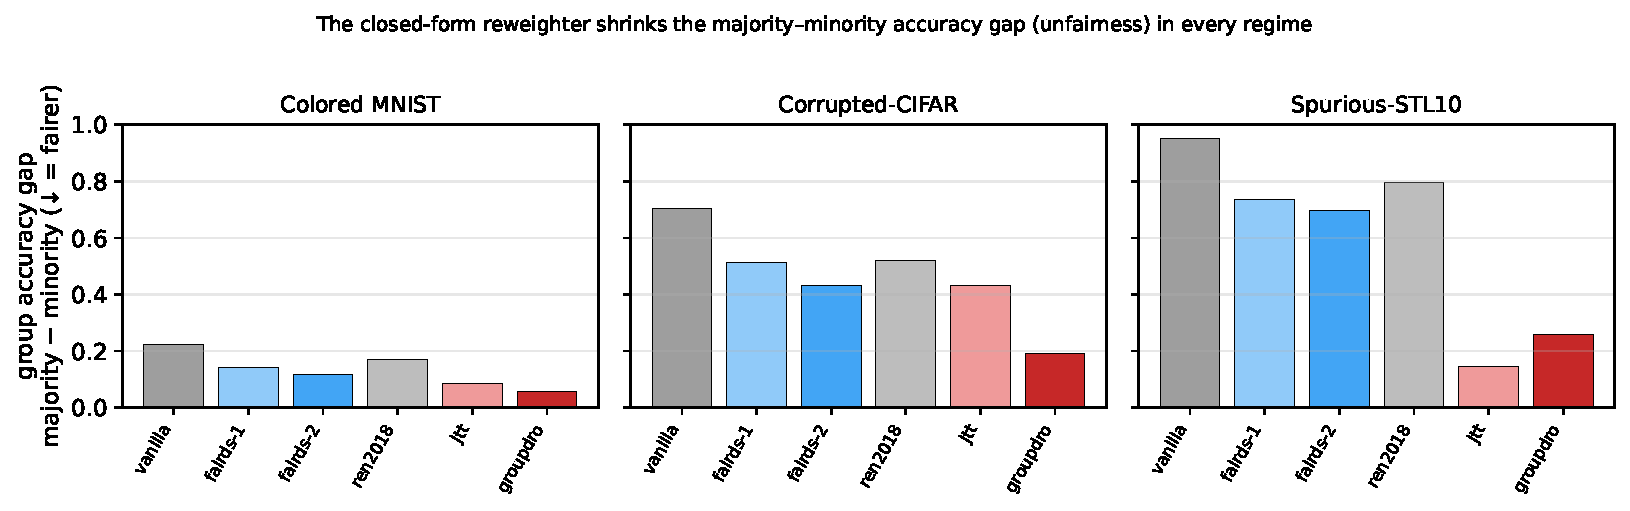
\includegraphics[width=0.99\columnwidth]{figures/fig_disparity.pdf}
\caption{\textbf{Unfairness (group accuracy gap), lower is fairer.} The
closed-form reweighter shrinks the majority--minority gap below ERM, Fairds-1, and
the bi-level baseline in all three regimes.}
\label{fig:disparity}
\end{figure}

\subsection{Why it works: the bias signal is the residual}
\label{sec:residual}
Is the second-order term a real bias signal or just smoothing? We build five arms
that share $\phi^{(1)}$ but treat the residual $r$ differently: \emph{phi1}
(first order), \emph{parallel} (shrinkage only), \emph{residual-real}
($\phi^{(1)}{-}\alpha r$), \emph{residual-shuffle} ($r$ permuted within
class$\times\phi^{(1)}$ bins), and \emph{sign-flip}. The order is unambiguous:
\textbf{real $>$ shuffle $>$ parallel}, and sign-flip collapses
(Figure~\ref{fig:residual}). On CIFAR, real beats shuffle by $+5.9$~pp
($p{=}0.0015$, 20 seeds) and the shrinkage arm by $+9.2$~pp. If $r$ were noise,
shuffling it within matched bins would not matter --- but it does. So the
bias-correcting signal is a real, sample-specific direction, not smoothing.

\begin{figure}[t]
\centering
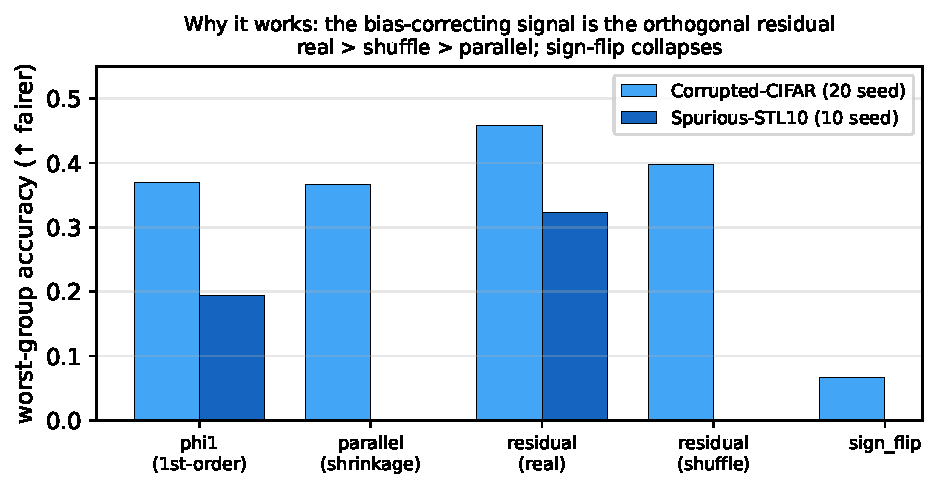
\includegraphics[width=0.94\columnwidth]{figures/fig_residual.pdf}
\caption{\textbf{Mechanism.} The orthogonal residual of the cross-term carries the
bias-correcting signal: real $>$ shuffle $>$ parallel; sign-flip collapses.}
\label{fig:residual}
\end{figure}

\paragraph{Controlled probe.}
On a controlled spurious-feature MLP (one strongly label-correlated feature in the
majority group), Fairds-2 assigns \emph{lower} Shapley values to majority than
minority examples (Mann--Whitney $U(\mathrm{maj}{<}\mathrm{min})$,
$p{=}1.89\times10^{-8}$ at ratio $0.9$), and $\Delta\phi$ falls as imbalance
grows. This is the bias-mitigation mechanism, seen directly: the cross-term
penalizes majority gradients aligned with the validation curvature.

\subsection{Demographic fairness: structured vs diffuse}
\label{sec:demographic}
Does this help \emph{real} demographic bias? It depends on whether the bias is
structured. Table~\ref{tab:demo} tests two kinds. On \textbf{CelebA} --- predict
Blond\_Hair with gender (Male) as the sensitive group; blond strongly correlates
with female, so blond-male is the tiny minority --- the bias is structured (one
dominant attribute in image space), and Fairds works strongly: worst-group
(blond-male) accuracy rises $0.20{\to}0.72$ ($+51$~pp, $p{=}0.002$, 10 seeds), the
equalized-odds gap falls $0.38{\to}0.16$, and overall accuracy \emph{improves}. It
nearly matches the bi-level baseline (Ren2018 worst $0.79$). On \textbf{Adult} and
\textbf{COMPAS} --- tabular bias spread over many weakly informative features ---
Fairds keeps accuracy but barely moves DP/EO, and the bi-level method is fairer.
The contrast is the point: the closed-form Shapley signal needs a \emph{structured}
bias to fire. It is a fairness tool for structured demographic bias --- even on
real faces --- not a general tabular debiaser.

\begin{table}[t]
\centering\footnotesize
\setlength{\tabcolsep}{4pt}
\begin{tabular}{llcccc}
\toprule
data & method & worst$\uparrow$ & DP$\downarrow$ & EO$\downarrow$ & acc \\
\midrule
CelebA  & Vanilla          & 0.20 & 0.237 & 0.381 & 0.773 \\
(image) & \textit{Fairds-2}& \textbf{0.72} & 0.213 & 0.158 & 0.856 \\
        & Ren2018          & 0.79 & 0.209 & \textbf{0.129} & 0.856 \\
\midrule
Adult   & Vanilla          & 0.80 & 0.196 & 0.117 & 0.837 \\
(tab.)  & \textit{Fairds-2}& 0.80 & 0.189 & 0.127 & 0.835 \\
        & Ren2018          & 0.78 & \textbf{0.175} & \textbf{0.102} & 0.819 \\
\midrule
COMPAS  & Vanilla          & 0.66 & 0.240 & 0.226 & 0.667 \\
(tab.)  & \textit{Fairds-2}& 0.66 & 0.239 & 0.244 & 0.671 \\
        & Ren2018          & 0.67 & \textbf{0.231} & 0.241 & 0.681 \\
\bottomrule
\end{tabular}
\caption{\textbf{Demographic fairness.} On \textbf{CelebA} (structured image bias)
Fairds lifts worst-group $+51$~pp and cuts EO sharply; on \emph{diffuse} tabular
data (Adult, COMPAS) it barely moves worst-group, DP, or EO --- the mechanism needs
structured bias.}
\label{tab:demo}
\end{table}

\section{Discussion and Conclusion}

Closed-form data valuation can make training fairer, \emph{within a characterized
regime}. The second-order Shapley cross-term down-weights the biased-majority
examples through its orthogonal residual --- a real, per-sample direction --- and
this raises worst-group accuracy and shrinks the majority--minority gap across
color, texture, and natural-image bias. The effect is strong when the bias is
structured (one dominant attribute) and weak when it is diffuse, as in tabular
demographic data, where a bi-level reweighter is the better tool. A further property is the
\emph{fairness--accuracy trade-off}: Fairds improves group fairness while
\emph{preserving} overall accuracy, whereas the bi-level reweighter trades
accuracy for fairness (Table~\ref{tab:demo}). Closed-form valuation thus gives a
distinct operating point --- moving toward fairness at almost no accuracy cost ---
which is attractive when accuracy must be kept and group labels are unavailable. The method is
not the fairest overall: two-stage (JTT) and group-label (GroupDRO) methods are
stronger, and the second-order variant costs ${\sim}7.7\times$ vanilla wall-clock
(the first-order variant, $4.3\times$, is cheaper than the bi-level baseline). Its
value is conceptual: a single-pass, closed-form valuation whose curvature term
provably carries a usable bias-mitigation signal. \textbf{Limitations:} (i) not
state-of-the-art fairness; (ii) second-order overhead; (iii) each image benchmark
isolates one biased attribute; (iv) the diffuse-bias failure is diagnosed
empirically, not proven; (v) the anchor needs group balance at construction,
though not in the update. Reducing the overhead and extending the mechanism to
diffuse bias are the natural next steps.

\section{Broader Impact}
Our goal is fairness, and the method is meant to \emph{reduce}, not certify,
unfairness. Two points matter for responsible use. First, the gains are real but
bounded: the reweighter raises worst-group accuracy and shrinks the group gap when
the bias is structured, yet barely moves demographic-parity or equalized-odds on
diffuse tabular data. It should therefore not be deployed as a sole fairness
guarantee, and group-label methods remain preferable when that supervision is
available. Second, the balanced anchor uses group labels at construction time
(though never in the model update); practitioners must check that those labels are
themselves trustworthy and that the chosen groups are the ones that matter. Used
within its scope --- a cheap, label-free training-time signal that keeps
structured bias out of the model --- the method complements rather than replaces
existing fairness tools.

\clearpage
\bibliography{references}

\end{document}
